\documentclass[WHATMANUAL.tex]{subfiles}

\begin{document}

\chapter[Hydrogeological characterization of the regional bedrock aquifer confinement conditions in Monteregie Est]{Hydrogeological characterization of the regional bedrock aquifer confinement conditions in Monteregie Est\footnotemark}\label{app:confinement_cond_in_MontEst}

\footnotetext{This work has been produced with the participation of Dr. René Lefebvre at INRS-ETE, 490 rue de la Couronne, Quebec City, Quebec, Canada.}


\section{methodology}

The water level was monitored in 44 observation wells during the PACES project in Monteregie Est for a period of approximately two years. The vast majority of the wells were installed in the regional fractured bedrock aquifer. Daily weather data for 32 weather stations in and around the Monteregie Est area were also retrieved from the Canadian Daily Climate Database (CDCD) with the software WHAT for the years 2000 to 2012. Missing values in the weather time series were also estimated with WHAT to produce gapless meteorological records of daily air temperature and precipitation.
 
Thiessen polygons were generated from the location of these 32 weather stations (see Figure~\ref{fig:Thiessen_meteo_wells}) and the hydrographs were next produced with WHAT by selecting the weather data on the basis of these polygons. These hydrographs were then inspected visually and grouped into three different classes according to the relative response of the water level to rainfall and snow melt events. These classes are interpreted in terms of confinement conditions of the regional bedrock aquifer: (1)~unconfined, (2)~confined, and (3)~semi-confined (or confined with regional influences from a nearby recharge area). The confinement conditions of the regional bedrock aquifer have thus been deducted at 35 sites in total since a fraction of the 44 wells are multi-level and are located side by side at the same location. Figure~\ref{fig:casTypes_hydrographs} shows typical hydrograph relating to the three conditions of confinement.

\begin{figure}[!ht]
\centering
\includegraphics[width=0.75\textwidth]{img/Thiessen_meteo_wells}
\caption[Locations of the observation wells and the weather stations in the Monteregie Est area.]{Locations of the observation wells (green dots) and the weather stations (blackheads) in the Monteregie Est area.}
\label{fig:Thiessen_meteo_wells}
\end{figure}

\section{Results}

The confinement conditions deducted from the well hydrographs were drawn on the map of confinement conditions of the regional bedrock aquifer that was produced based on the sequence and thickness of the surficial deposits \citep{carrier_portrait_2013}. Figure~\ref{fig:CONFINEMENTetPUITS} shows that the confinement conditions of the regional bedrock aquifer defined on the basis of the well hydrographs are generally consistent with those of the map of confinement conditions. This is an interesting result considering that the two approaches are completely independent. That is, the definition of the confinement conditions of the bedrock aquifer for both approaches stems from criteria based on physical quantities that are very different in nature: time series of groundwater levels in one case and spatial distribution of surficial deposits in the other. The confinement conditions deduced from the hydrographs come to validate the criteria used to produce the regional map of confinement conditions which were based on professional judgment and were therefore relatively arbitrary, even if they are logical according to regional conditions.

More specifically, the confinement conditions deducted from the well hydrographs are also consistent with the four different hydrogeological contexts defined in the study area. These contexts are represented by thick dashed lines in Figure~\ref{fig:CONFINEMENTetPUITS} and were defined based on the physiography, the spatial coverage of surficial deposits, and the geological rock formations of the Monteregie Est region. A discussion relative to each context is presented in some details in the following paragraphs.

\begin{figure}[!hb]
\centering
\includegraphics[height=0.85\textheight]{img/CasTypes.png}
\caption[Typical hydrographs relating to the three classes that were considered in the analysis of the confinement conditions of the regional bedrock aquifer in the Monteregie Est area, Quebec, Canada.]{Typical hydrographs relating to the three classes that were considered in the analysis of the confinement conditions of the regional bedrock aquifer in the Monteregie Est area, Quebec, Canada: (top) confined, (middle) semi-confined (or confined with regional influences), and (bottom) unconfined.}
\label{fig:casTypes_hydrographs}
\end{figure}

\begin{figure}
\centering
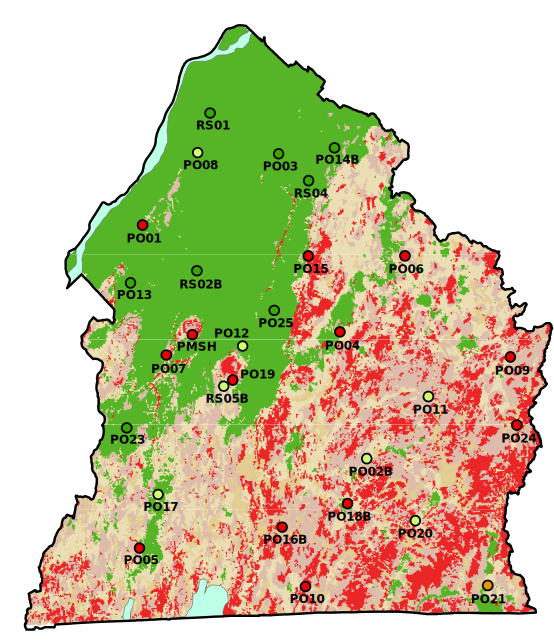
\includegraphics[height=0.85\textheight]{img/CONFINEMENTetPUITS}
\caption[Confinement conditions deducted from the well hydrographs compared to the map of confinement conditions of the regional bedrock aquifer.]{Confinement conditions deducted from the well hydrographs (dots) compared to the map of confinement conditions of the regional bedrock aquifer. The colors indicate the conditions of confinement of the aquifer, both for the map and the well symbols: green for captive, red for free, and other tones for semi-captive.}
\label{fig:CONFINEMENTetPUITS}
\end{figure}

\newpage

\paragraph{St-Laurent Lowlands} Observation wells representative of captive conditions are found exclusively in the St-Laurent Lowlands, particularly in the northern part where a thick layer of marine clay is present. The interpretation of the hydrographs is also consistent with the confinement conditions of the aquifer of this area at a more local scale. For example, the well PO01 represents adequately the small recharge area that is located in the north-western part of the St-Laurent Lowlands, where the sediments are coarser and their thickness less important. Moreover, the well PO08, located at a distance of $\sim$20~km from the well PO01 and at less than 7~km from the limit of the recharge zone, is characterized by water level that varies significantly on a seasonal basis, in spite of the thick layer of clay (more than 25 m) covering the rock at this location. These piezometric variations are most probably due to the influence of the nearby recharge area. The southern part of the St-Laurent Lowlands is characterized by wells representative of captive, semi-captive, and unconfined conditions that are distributed consistently with the nature and thickness of the surficial deposits.

\paragraph{Appalachian Foothills} This context is characterized by wells that are exclusively representative of unconfined conditions. This is even the case for the well PO18 where the rock is covered by more than 40~m of surficial sediments, mainly gravel, sand and silt. It is not clear if the strong correlation observed between the water level fluctuations and the rainfall and snow melt events are due to direct recharge at the PO18 location specifically, or is an hydraulic influence of recharge in the bedrock aquifer around the depression that is covered by a much thinner layer of surficial sediments. The calculation of the barometric response function for this well would be of a great help to answer this particular question.

\paragraph{Appalachian Highlands} This context is characterized by wells indicating conditions ranging from unconfined to semi-confined. These results represent adequately the discontinuous cover of the surficial deposits in this area. The fact that there is no well showing captive conditions, despite the important thickness of the surficial sediments in some valleys, suggests a significant hydraulic influence of recharge areas of the bedrock aquifer located in elevation on areas located in topographic depressions (valleys). The well PO20 that has been classified as semi-confined with more than 24~m of surficial sediments is a good example.

\paragraph{Monteregian Hills} The wells located directly on the Monteregian Hills are representative of unconfined conditions, while the ones located on their periphery range from unconfined to semi-captive conditions. This situation is particularly well represented by the wells PO19, PO12, and RS05b located near Mont Rougemont: the well PO19, located directly on Mont Rougemont, indicates unconfined conditions, while the wells PO12 and RS05b indicate semi-confined conditions. This result is especially interesting for PO12 where the rock is covered with a thick layer of clayey silt of more than 23~m. The fluctuations of the water level in well PO12 represent most probably the influence of the rocky aquifer recharge on the Monteregian Hills. These hills are supposed to be preferential recharge areas in the region and these results are in agreement with this hypothesis.

\newpage

\section{Conclusion}

The qualitative visual interpretation of the relative response of the water levels to rainfall and snow melt events has provided an independent validation of the criteria, based on the thickness and nature of the overburden, that were used to produce the map of confinement conditions of the regional bedrock aquifer. Actually the containment level of the bedrock aquifer is not clearly defined into three distinct classes, but varies over a continuous range of conditions ranging from perfectly free to completely confined.

Moreover, it is not possible to clearly distinguish between wells that are in semi-confined condition and wells for which the water level are hydraulically influenced by nearby recharge areas. It is also important to mention that this approach worked well in the hydrogeological context of the Monteregie Est because the water table was relatively close to the ground surface and the recharge events were consequently clearly defined in the hydrographs. The application of a similar approach to a study area with a deeper water table would have required data on a longer period than two years to be fully applicable.

A complementary analysis to this approach would consist in the calculation of the barometric response function of the wells using measurement of water level and atmospheric pressure with a high temporal resolution (at least 4 measurements per hour). This technique is very useful to characterized the confinement conditions of a well at the local scale. The application of this technique for the Monteregie Est area is presented in Appendix~C.

\end{document}